\documentclass[12pt]{article}

\usepackage{sbc-template}
\usepackage{graphicx,url}
\usepackage{amsmath}
\usepackage[utf8]{inputenc}
\usepackage[brazil]{babel}

\sloppy

\title{Gamificação de testes traduzida em níveis de prompt:\\ uma replicação
  adaptada a modelos de IA geradores de código}

\author{Kaike Carvalho,\inst{1}, Sergio Murilo Cardoso Valentini\inst{2}, Hebert Willy Cardoso do Carmo\inst{3}}

\address{CAMPUS CAMPO MOURÃO -- Universidade Tecnológica Federal do Paraná 
(UTFPR)\\
  Via Rosalina Maria dos Santos, 1233 --  Campo Mourão -- PR -- Brasil
\nextinstitute
  Departamento Acadêmico de Computação (DACOM)\\
  Universidade Tecnológica Federal do Paraná (UTFPR) -- Campo Mourão, PR -- Brasil
  \email{carvalhokaike69@gmail.com, sergiomurilo-cardoso@hotmail.com,}
  \email{hebert@alunos.utfpr.edu.br}
}


\begin{document}

\maketitle

\begin{resumo}
  Este trabalho replica o estudo \emph{Gamifying Testing in IntelliJ: A
  Replicability Study} \cite{straubinger2025}, no qual a gamificação de testes
  foi avaliada com 174 participantes humanos usando o plugin IntelliGame no
  IntelliJ IDEA. A adaptação substitui os participantes humanos por três modelos
  de IA geradores de código (Gemini 2.5 Flash, GPT-OSS-120B e Llama 3.3 70B) e
  reinterpreta a variável independente: em vez de gamificação (presente ou
  ausente), varia-se o nível de detalhe do prompt, traduzindo os incentivos
  implícitos das conquistas do IntelliGame em instruções explícitas de
  qualidade. Em um desenho fatorial 3$\times$3 com dez execuções por célula (90
  ao todo), mede-se a qualidade estática dos artefatos gerados. Os resultados
  mostram que o \emph{modelo} é o fator dominante e que o detalhe do prompt
  aumenta significativamente o número de testes (efeito grande), enquanto a
  tensão quantidade \emph{vs.} qualidade observada nos humanos quase não
  reaparece nas IAs.
\end{resumo}

\section{Introdução}

A gamificação, o uso de elementos de jogos em contextos não lúdicos, tem
sido investigada como estratégia para aumentar o engajamento e a produtividade
em atividades de engenharia de software tradicionalmente pouco motivadoras,
como a escrita de testes. O estudo de \cite{straubinger2025} replicou e validou
os efeitos do \emph{IntelliGame}, um plugin de gamificação para o IntelliJ
IDEA, em um experimento controlado com 174 participantes divididos em grupo
\emph{treatment} (com gamificação) e grupo de controle (sem). Os autores
observaram que o grupo gamificado escreveu mais testes, executou-os com mais
frequência e produziu implementações de melhor qualidade.

Paralelamente, modelos de linguagem de larga escala (LLMs) passaram a gerar código e
testes de forma cada vez mais competente, e deslocaram parte da atividade de
teste do desenvolvedor humano para sistemas automáticos. Surge a questão: os
efeitos atribuídos à gamificação, escrever mais testes, buscar cobertura,
aplicar análise de valores-limite (BVA) e casos de borda, tratar robustez,
também se manifestam quando o ``participante'' é um modelo de IA? Como uma IA
não interage com uma IDE nem responde a conquistas ao longo de uma sessão, a
gamificação no sentido original não é diretamente aplicável. Propõe-se, então,
traduzir o estímulo da gamificação para o único canal de controle disponível
sobre um modelo generativo: o prompt.

Este artigo apresenta tal replicação. Não se trata de uma réplica literal, mas
de uma replicação conceitual adaptada: o fenômeno investigado (o efeito de um
estímulo de qualidade sobre o comportamento de teste) é preservado, enquanto o
agente e o mecanismo de estímulo são substituídos. As contribuições são: (i) a
descrição do estudo a ser replicado e dos objetivos da replicação; (ii) três
questões de pesquisa reformuladas (RQ1$'$--RQ3$'$); (iii) o protocolo
experimental, explicitando o que é mantido e o que é novo; e (iv) a
\emph{execução} das 90 rodadas, com a análise estatística que responde às
questões de pesquisa.

\section{O estudo a ser replicado}

O estudo original \cite{straubinger2025}, publicado nos \emph{Proceedings of
the ACM on Software Engineering} (ISSTA 2025), é em si uma replicação: ele
generaliza achados anteriores sobre gamificação de testes para um novo contexto, a linguagem TypeScript e um grupo maior de participantes. O desenho é um
experimento controlado de dois grupos. A variável independente é a presença da
gamificação: o grupo \emph{treatment} usa o plugin IntelliGame, cujas
conquistas e \emph{feedback} incentivam implicitamente bons comportamentos de
teste. o grupo de controle trabalha no mesmo ambiente, sem o plugin. A tarefa
consiste em implementar e testar um conjunto de funções de manipulação de datas
(baseadas na biblioteca \texttt{date-fns} \cite{datefns}) em uma janela de
tempo fixa.

As variáveis dependentes incluem o comportamento de teste (quantidade de testes
escritos, frequência de execução, uso de ferramentas de cobertura e
\emph{debug}), a qualidade da suíte (cobertura de linha e \emph{branch},
\emph{mutation score}), a funcionalidade do código produzido e a percepção dos
participantes coletada por questionário. O estudo organiza-se em sete questões
de pesquisa (RQ1--RQ7) e conclui que a gamificação, via IntelliGame, impacta
positivamente o comportamento de teste e o engajamento, embora aponte uma
tensão entre quantidade e qualidade: o grupo gamificado também produziu mais
\emph{test smells} e mais falhas associadas a data, hora e fuso. O pacote de
replicação do estudo (código, \emph{scripts} de análise em R, \emph{surveys} e
dados brutos) é público e serviu de base para esta adaptação.

\section{Objetivos da replicação}

O objetivo geral é verificar se o efeito documentado por \cite{straubinger2025}, um estímulo de qualidade melhora o comportamento de teste, persiste
quando o agente produtor de testes é um modelo de IA, e quando o estímulo é
entregue como detalhamento do prompt em vez de gamificação. Especificamente,
busca-se:

\begin{enumerate}
  \item Reinterpretar a variável independente do estudo original (gamificação
  presente ou ausente) como um gradiente de detalhe de prompt (básico,
  intermediário e completo), no qual o prompt completo \emph{verbaliza}
  explicitamente os comportamentos que a gamificação induzia de forma
  implícita.
  \item Medir, por métricas estáticas e automatizáveis atribuíveis ao modelo,
  as variáveis dependentes que sobrevivem à substituição do humano pela IA
  (qualidade da suíte, funcionalidade e robustez).
  \item Avaliar se a tensão quantidade \emph{vs.} qualidade observada no grupo
  \emph{treatment} humano reaparece sob prompts mais detalhados ou em
  determinados modelos.
\end{enumerate}

Por construção, excluem-se as questões do estudo original que dependem de
comportamento interativo humano, dos níveis de conquista do plugin ou de
questionário (RQ1, RQ3, RQ5 e RQ7): uma IA gera o artefato de uma só vez, sem
sessão interativa a observar, sem plugin a gerar relatórios de conquista e sem
participante humano para responder ao \emph{survey}. As demais (RQ2, qualidade
da suíte; RQ4, funcionalidade; RQ6, qualidade e robustez) são mensuráveis
estaticamente e fundamentam as questões reformuladas.

\section{Questões de pesquisa}

A replicação organiza-se em torno de três questões de pesquisa, análogas às
dimensões mensuráveis do estudo original:

\begin{itemize}
  \item \textbf{RQ1$'$: Efeito do detalhe do prompt.} O nível de detalhe do
  prompt (básico, intermediário, completo) influencia a qualidade da suíte e do
  código gerados? \emph{(análogo do efeito da gamificação)}
  \item \textbf{RQ2$'$: Variação entre modelos.} O efeito do prompt é
  consistente entre os modelos de IA ou depende do modelo? \emph{(análogo do
  papel da população de participantes)}
  \item \textbf{RQ3$'$: Quantidade \emph{vs.} qualidade e robustez.} Prompts
  mais detalhados (ou certos modelos) geram testes mais minuciosos porém mais
  frágeis? \emph{(reaproveita o achado central do estudo original: mais testes,
  porém mais \emph{test smells} e falhas de data e hora)}
\end{itemize}

\section{Desenho da replicação}

\subsection{Visão geral}

Adota-se um desenho fatorial 3$\times$3. O \emph{Fator~1} é o nível de prompt
(básico, intermediário, completo); o \emph{Fator~2} é o modelo de IA (três
modelos distintos, cumprindo o papel da ``população de participantes''). Isso
resulta em nove células; cada célula é executada $K=10$ vezes, totalizando 90
execuções. A repetição é necessária porque modelos de IA são estocásticos: a
mesma combinação (modelo, prompt) produz artefatos distintos a cada execução.
Reportar-se-á mediana e distribuição por célula, e não um valor único de
$N=1$.

\begin{table}[ht]
\centering
\caption{Os três níveis de prompt e seu análogo no estudo original.}
\label{tab:prompts}
\begin{tabular}{p{2.3cm} p{5.1cm} p{4.5cm}}
\hline
\textbf{Nível} & \textbf{O que acrescenta} & \textbf{Análogo no original} \\
\hline
Básico & Apenas o enunciado das 11 funções + escrever testes & Piso, sem equivalente direto \\
Intermediário & README, JSDoc, \texttt{test.ts}, comandos, \texttt{main.ts}, documentação MDN & Grupo de controle (ambiente, sem incentivo) \\
Completo & Cobertura alta, BVA/casos de borda, robustez data/hora, TDD, janela de 150~min & Grupo \emph{treatment} (IntelliGame) \\
\hline
\end{tabular}
\end{table}

A Tabela~\ref{tab:prompts} resume a tradução do estímulo: a gamificação não foi
abandonada, e sim traduzida de ``\emph{nudge} motivacional'' para ``instrução
explícita'', em que o prompt completo declara os mesmos objetivos que as
conquistas do IntelliGame incentivavam de forma implícita.

\subsection{O que é mantido e o que é novo}

\textbf{Mantém-se} do estudo original a \textbf{tarefa} (as 11 funções derivadas
de \texttt{date-fns}, em TypeScript com Jest), as \textbf{métricas de qualidade}
(número de testes, cobertura de linha e \emph{branch}, \emph{mutation score},
funcionalidade pela \emph{golden-suite} e \emph{test smells}, espelhando RQ2, RQ4
e RQ6), a \textbf{abordagem estatística} (não-paramétrica, com correção de Holm) e
o \textbf{achado a testar} (mais estímulo gera mais e melhores testes, com
possível custo em fragilidade). \textbf{É novo:} o \textbf{agente} (modelos de IA
no lugar dos 174 participantes humanos); a \textbf{variável independente} (o nível
de detalhe do prompt no lugar da gamificação, com um nível básico abaixo do
controle como piso); a \textbf{natureza da medição} (qualidade estática do
artefato gerado de uma só vez, sem IDE nem plugin); e o \textbf{tratamento da
estocasticidade} ($K=10$ por célula e relato por distribuição no lugar do $N$ de
participantes).

\section{Metodologia}

\subsection{Os três níveis de prompt}

O estímulo é operacionalizado por três prompts de detalhe crescente
(Tabela~\ref{tab:prompts}), todos entregues junto do projeto-base. O
\textbf{básico} traz só o enunciado (piso, sem apoio nem meta de qualidade); o
\textbf{intermediário} acrescenta o ambiente do projeto (JSDoc como
especificação, \texttt{test.ts}, comandos \texttt{npm test}, \texttt{main.ts} e a
documentação MDN \emph{offline}), correspondendo ao grupo de controle; o
\textbf{completo} adiciona objetivos de qualidade \emph{verbalizados} (cobertura
alta de linha/\emph{branch}, BVA e casos de borda, robustez a data/fuso/\emph{locale},
TDD e janela de 150~min), declarando explicitamente o que as conquistas do
IntelliGame induziam de forma implícita no grupo \emph{treatment}.

\subsection{Modelos, projeto-base e métricas}

Os três modelos são o \textbf{Gemini 2.5 Flash} (Google AI Studio), o
\textbf{GPT-OSS-120B} e o \textbf{Llama 3.3 70B Instruct} (ambos via
OpenRouter), invocados por API com parâmetros fixos por célula para que a
variabilidade observada seja do modelo, e não da configuração. Cada execução
parte de uma cópia \emph{pristina} do projeto-base (11 funções derivadas de
\texttt{date-fns} em TypeScript com Jest; a auxiliar \texttt{toDate} já
implementada). A pontuação é totalmente estática e atribuível ao artefato:
número de testes (contagem de \texttt{test(}/\texttt{it(}), cobertura de linha e
\emph{branch} (Jest com \texttt{json-summary}), \emph{mutation score} (StrykerJS
\cite{stryker}), funcionalidade pela \emph{golden-suite} de referência ($\approx
60$ testes, usada apenas para \emph{scoring} e nunca entregue ao modelo), razão
de testes próprios que falham e razão de \emph{test smells}. A execução fixa
\texttt{TZ=UTC} para tornar a pontuação determinística entre máquinas.

\subsection{Análise estatística}

Cada célula (modelo $\times$ prompt) é executada $K=10$ vezes; reporta-se mediana
e distribuição, não um valor único. Comparam-se os grupos com Kruskal--Wallis
seguido de Mann--Whitney pareado com correção de Holm ($\alpha = 0{,}05$),
espelhando o teste de Wilcoxon--Mann--Whitney do estudo original. O tamanho de
efeito é medido pelo $\delta$ de Cliff, e a interação prompt $\times$ modelo, pelo
teste de Scheirer--Ray--Hare (SRH).

\section{Resultados}

A Tabela~\ref{tab:medianas} apresenta as medianas por célula e a
Figura~\ref{fig:boxplots} mostra a distribuição das métricas por nível de prompt
e modelo.

\begin{table}[ht]
\centering
\caption{Medianas por modelo $\times$ nível de prompt (B = básico, I = intermediário, C = completo). Cob.\ = cobertura; Mut.\ = \emph{mutation score}; Falha = razão de testes próprios que falham. O \emph{mutation score} é a mediana sobre os runs com suíte passante (6 a 10 por célula, pois o StrykerJS exige a suíte verde).}
\label{tab:medianas}
\small
\resizebox{\textwidth}{!}{%
\begin{tabular}{l ccc ccc ccc}
\hline
 & \multicolumn{3}{c}{\textbf{Gemini 2.5 Flash}} & \multicolumn{3}{c}{\textbf{GPT-OSS-120B}} & \multicolumn{3}{c}{\textbf{Llama 3.3 70B}} \\
\textbf{Métrica} & B & I & C & B & I & C & B & I & C \\
\hline
Nº de testes      & 82{,}5 & 90{,}5 & 133 & 22 & 23{,}5 & 49{,}5 & 11 & 22{,}5 & 23{,}5 \\
Cob.\ linha (\%)  & 98{,}8 & 98{,}7 & 98{,}8 & 95{,}9 & 97{,}9 & 98{,}3 & 93{,}2 & 93{,}8 & 93{,}9 \\
Cob.\ branch (\%) & 91{,}2 & 90{,}5 & 91{,}2 & 55{,}8 & 72{,}2 & 76{,}9 & 32{,}3 & 32{,}1 & 50{,}0 \\
Mut.\ (\%)        & 76{,}3 & 76{,}9 & 77{,}0 & 90{,}7 & 91{,}0 & 100 & 63{,}9 & 87{,}3 & 85{,}0 \\
Golden (de 60)    & 58 & 58 & 58 & 58 & 57 & 58 & 57 & 54{,}5 & 54{,}5 \\
Falha (razão)     & 0{,}00 & 0{,}00 & 0{,}02 & 0{,}00 & 0{,}00 & 0{,}02 & 0{,}09 & 0{,}05 & 0{,}11 \\
\hline
\end{tabular}%
}
\end{table}

\begin{figure}[ht]
\centering
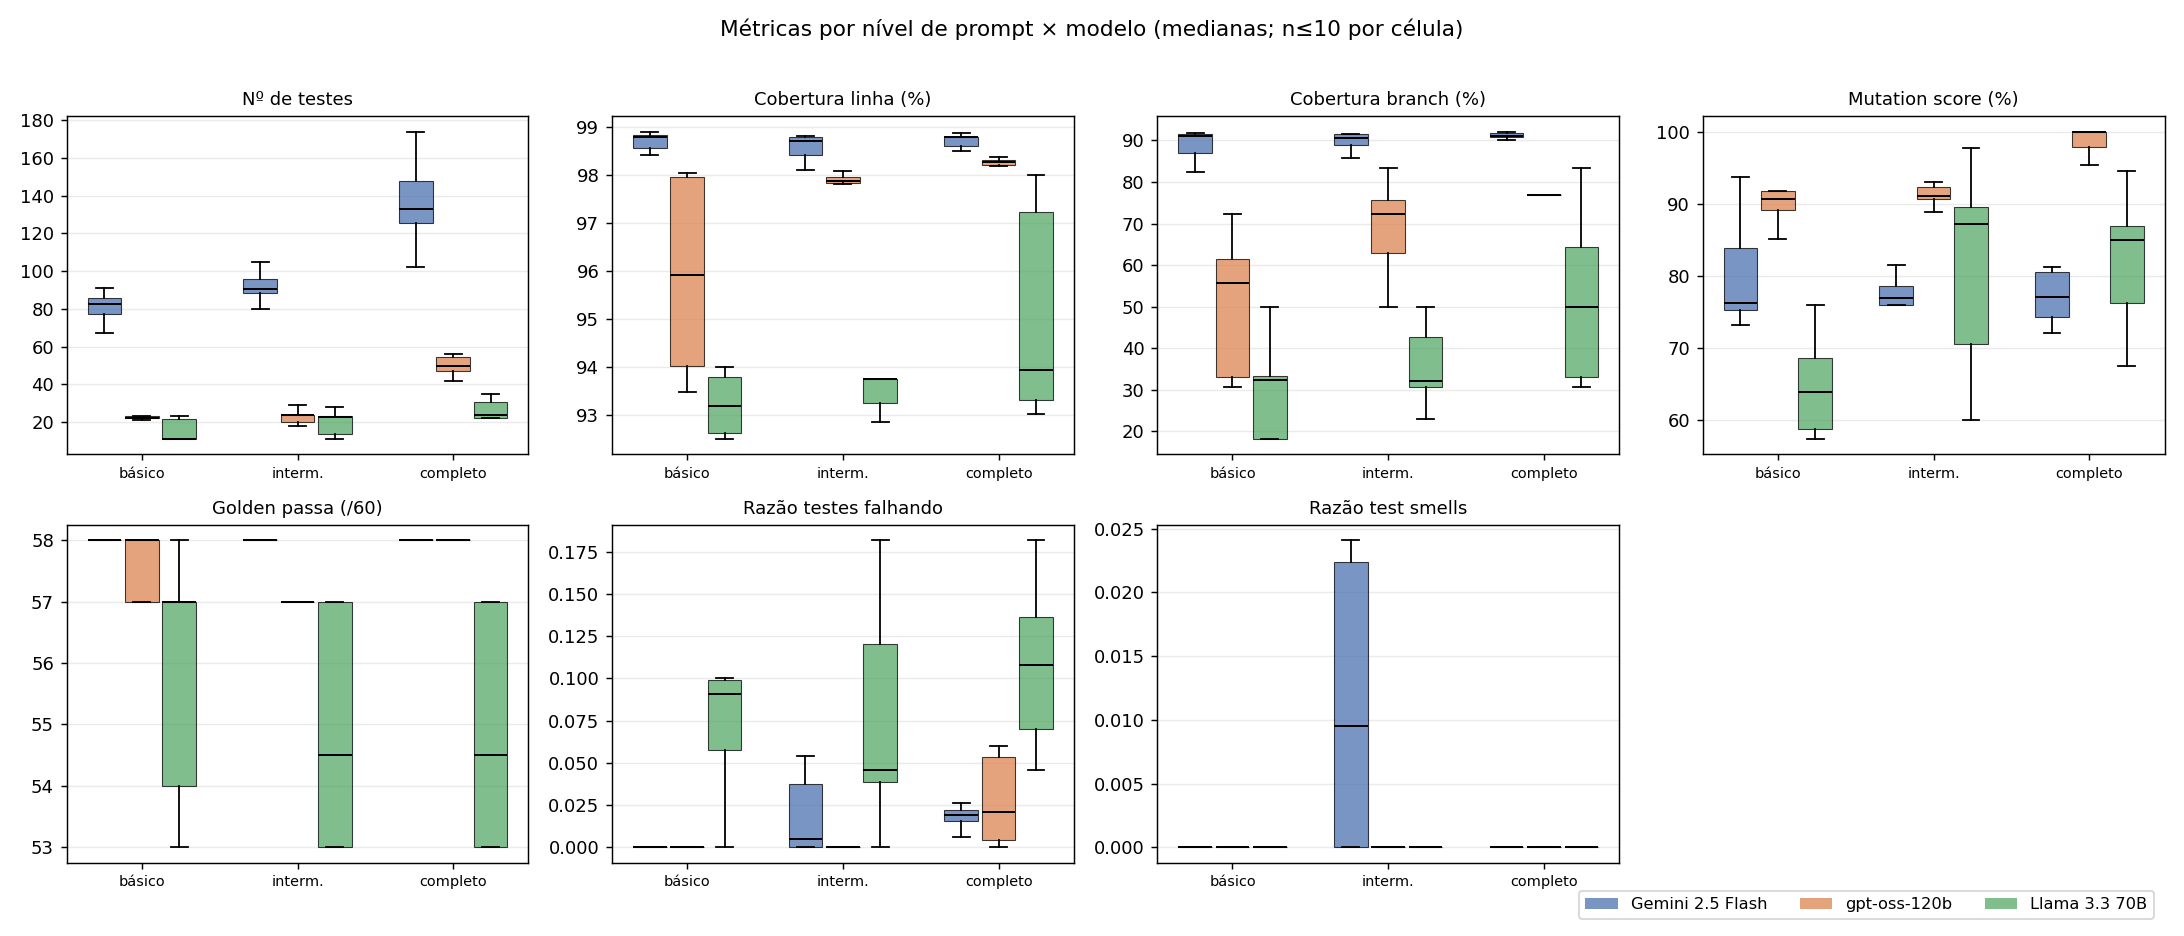
\includegraphics[width=0.80\textwidth]{boxplots.png}
\caption{Distribuição das métricas por nível de prompt (cor) e modelo (eixo).}
\label{fig:boxplots}
\end{figure}

\paragraph{RQ1$'$: efeito do detalhe do prompt.} Detalhar o prompt aumenta o
número de testes de forma significativa: comparando todos os modelos, do básico
ao completo, $p_{\text{Holm}} = 0{,}005$ com $\delta = -0{,}48$ (efeito grande).
O efeito é mais nítido no Gemini (de 82{,}5 para 133 testes) e no GPT-OSS (de 22
para 49{,}5), e acompanha melhora de cobertura de \emph{branch} e \emph{mutation}
no GPT-OSS (de 55{,}8\% para 76{,}9\% e até 100\%). No Gemini a cobertura já está
saturada (linha $\approx 98{,}8\%$, \emph{branch} $\approx 91\%$), de modo que o
prompt afeta sobretudo a quantidade. A cobertura de linha global não varia
significativamente com o prompt ($p_{\text{Holm}} > 0{,}13$).

\paragraph{RQ2$'$: variação entre modelos.} O \emph{modelo} é o fator
dominante. As diferenças entre modelos são significativas e grandes em quase
todas as métricas: para o número de testes, $\delta = 1{,}000$ entre o Gemini e
cada um dos demais ($p < 0{,}0001$); o teste SRH aponta $p_{\text{modelo}} \approx
0{,}0000$ para todas as métricas, contra um efeito de prompt bem menor. O efeito
do prompt é \emph{dependente do modelo} (forte em Gemini, fraco em Llama), mas a
direção é consistente, e não há interação prompt $\times$ modelo relevante
($p_{\text{inter}} > 0{,}47$), exceto o \emph{mutation score} no limiar
($p = 0{,}049$).

\paragraph{RQ3$'$: quantidade \emph{vs.} qualidade e robustez.} A tensão
observada nos humanos \emph{quase não reaparece}. A razão de \emph{test smells} é
$\approx 0$ em todos os modelos e níveis. A razão de testes próprios que falham
sobe levemente com o prompt completo ($p_{\text{Holm}} = 0{,}003$,
$\delta = -0{,}48$), concentrada no Llama (0{,}11), que também tem a menor
cobertura e o pior desempenho na \emph{golden-suite} (54,5/60). Ou seja, escrever
mais testes não degradou a qualidade nos modelos mais capazes; só o mais fraco
mostrou sinal de fragilidade.

\section{Ameaças à validade}

As ameaças à validade espelham a seção 3.7 do estudo original, ajustada à substituição de humanos por IA.
\textbf{Validade de construto:} o nível de detalhe do prompt é um \emph{proxy} da
gamificação, não um equivalente perfeito; instrução explícita não é idêntica a um
incentivo implícito por conquistas. As RQ1, RQ3, RQ5 e RQ7 do original foram
excluídas por construção, pois dependem de comportamento interativo, de níveis de
conquista do plugin ou de questionário, inexistentes quando o agente gera o
artefato de uma só vez. \textbf{Validade interna:} a \texttt{date-fns} é pública e
popular, logo os modelos podem tê-la visto no treino, o experimento mede geração
\emph{condicionada ao prompt}, não capacidade ``do zero''; parâmetros foram
fixados por célula e a \emph{golden-suite} nunca foi exposta ao modelo (correções
de \emph{setup} como \texttt{TZ=UTC} garantem reprodutibilidade).
\textbf{Validade de conclusão:} a estocasticidade é tratada com $K=10$ e relato
por distribuição, mas $K=10$ limita a potência para efeitos pequenos.
\textbf{Validade externa:} três modelos são uma amostra de conveniência e não
generalizam para ``IAs'' em geral; a tarefa tem poucos \emph{branches} por
natureza, limitando a variância de cobertura e \emph{mutation}; e o desenho não
captura uso interativo nem colaboração humano-IA.

\section{Conclusão}

A replicação adaptada mostra que o estímulo de qualidade, traduzido de
gamificação para detalhe de prompt, de fato aumenta a quantidade de testes
gerados (efeito grande) e confirma, no contexto de IA, o achado central de
\cite{straubinger2025}. No entanto, o \emph{modelo} escolhido pesa mais que o
prompt: Gemini e GPT-OSS respondem fortemente ao detalhamento, enquanto o Llama
pouco reage e apresenta a menor qualidade. Diferentemente dos humanos, as IAs
praticamente não exibiram a tensão quantidade \emph{vs.} qualidade. Como trabalho
futuro, propõe-se ampliar o conjunto de modelos, usar tarefas com mais ramos
condicionais e controlar a contaminação dos dados de treino, para fortalecer a
validade externa.

\bibliographystyle{sbc}
\bibliography{referencias}

\end{document}
